\documentclass{beamer}

\usepackage{beamerthemesplit}
\usepackage[utf8x]{inputenc}
\usepackage{pgf}
\usepackage{default}
\usepackage{url}
\usepackage{subfigure}
\usepackage{algorithmic} 
\usepackage{algorithm} 
\usepackage{amssymb}

\usetheme{Singapore}


%Define some commands for printing correct variables in math mode 
\newcommand{\av}{\textbf{a}}
\newcommand{\bv}{\textbf{b}}
\newcommand{\cv}{\textbf{c}}
\newcommand{\dv}{\textbf{d}}
\newcommand{\ev}{\textbf{e}}
\newcommand{\fv}{\textbf{f}}
\newcommand{\gv}{\textbf{g}}
\newcommand{\hv}{\textbf{h}}
\newcommand{\iv}{\textbf{i}}
\newcommand{\jv}{\textbf{j}}
\newcommand{\kv}{\textbf{k}}
\newcommand{\lv}{\textbf{l}}
\newcommand{\mv}{\textbf{m}}
\newcommand{\nv}{\textbf{n}}
\newcommand{\ov}{\textbf{o}}
\newcommand{\pv}{\textbf{p}}
\newcommand{\qv}{\textbf{q}}
\newcommand{\rv}{\textbf{r}}
\newcommand{\sv}{\textbf{s}}
\newcommand{\tv}{\textbf{t}}
\newcommand{\uv}{\textbf{u}}
\newcommand{\vv}{\textbf{v}}
\newcommand{\wv}{\textbf{w}}
\newcommand{\xv}{\textbf{x}}
\newcommand{\yv}{\textbf{y}}
\newcommand{\zv}{\textbf{z}}

\newcommand{\alphav}{\mbox{\boldmath$\alpha$}}
\newcommand{\betav}{\mbox{\boldmath$\beta$}}
\newcommand{\gammav}{\mbox{\boldmath$\gamma$}}
\newcommand{\xiv }{\mbox{\boldmath$\xi$}}
\newcommand{\muv}{\mbox{\boldmath$\mu$}}
\newcommand{\tauv}{\mbox{\boldmath$\tau$}}
\newcommand{\Omegam}{\mbox{\boldmath$\Omega$}}
\newcommand{\Lambdam}{\mbox{\boldmath$\Lambda$}}
\newcommand{\Sigmam}{\mbox{\boldmath$\Sigma$}}
\newcommand{\Gammam}{\mbox{\boldmath$\Gamma$}}
\newcommand{\Deltam}{\mbox{\boldmath$\Delta$}}
\newcommand{\Thetam}{\mbox{\boldmath$\Theta$}}
\newcommand{\Phim}{\mbox{\boldmath$\Phi$}}
\newcommand{\Pim}{\mbox{\boldmath$\Pi$}}

\newcommand{\diag}{\mbox{diag}}
\newcommand{\tr}{\mbox{tr}}
\newcommand{\card}{\mbox{card}}
\newcommand{\cov}{\mbox{cov}}
\newcommand{\sign}{\mbox{sign}}
\newcommand{\var}{\mbox{var}}
\newcommand{\st}{\mbox{s.t.}}
\newcommand{\rank}{\mbox{rank}}
\newcommand{\argmin}{\mbox{argmin}}
\newcommand{\argmax}{\mbox{argmax}}

\newcommand{\Am}{\textbf{A}}
\newcommand{\Bm}{\textbf{B}}
\newcommand{\Cm}{\textbf{C}}
\newcommand{\Dm}{\textbf{D}}
\newcommand{\Em}{\textbf{E}}
\newcommand{\Fm}{\textbf{F}}
\newcommand{\Gm}{\textbf{G}}
\newcommand{\Hm}{\textbf{H}}
\newcommand{\Imat}{\textbf{I}}
\newcommand{\Jm}{\textbf{J}}
\newcommand{\Km}{\textbf{K}}
\newcommand{\Lm}{\textbf{L}}
\newcommand{\Mm}{\textbf{M}}
\newcommand{\Nm}{\textbf{N}}
\newcommand{\Om}{\textbf{O}}
\newcommand{\Pm}{\textbf{P}}
\newcommand{\Qm}{\textbf{Q}}
\newcommand{\Rm}{\textbf{R}}
\newcommand{\Sm}{\textbf{S}}
\newcommand{\Tm}{\textbf{T}}
\newcommand{\Um}{\textbf{U}}
\newcommand{\Vm}{\textbf{V}}
\newcommand{\Wm}{\textbf{W}}
\newcommand{\Xm}{\textbf{X}}
\newcommand{\Ym}{\textbf{Y}}
\newcommand{\Zm}{\textbf{Z}}

%Use regular expression: (\[a-z])([^a-zA-Z])  -> \1v\2  to change old style macros 
\graphicspath{{./Figures/}}

\title{Statistics and the Analysis of Data\\ Lecture 1: Descriptive Statistics}
\author{Charanpal Dhanjal \\ \texttt{charanpal@gmail.com}} 
\institute{\'{E}cole des Ponts}
\date{\today}

\begin{document}

\frame{\titlepage}

\begin{frame}{Course Overview}
\begin{itemize}
\item Timetable 
\begin{itemize}
\item 8 lecture session of 2 hours
\item 4 exercise sessions of 2 hours
\item 1 exam of 2 hours 
\end{itemize}
\item Overview
\begin{itemize} 
\item Descriptive statistics - means, modes, standard deviation, histograms etc. 
\item Multivariate statistics - PCA, graphical models
\item Parametric statistics - parameter estimation, confidence intervals, hypothesis testing    
\item Multiple linear regression 
\end{itemize}
\end{itemize}
\end{frame}

\begin{frame}{Lecture Overview}
\begin{itemize} 
 \item What is statistics and motivation
\item Statistical measures - mean, median, spread 
\item Graphical representations of distributions - histograms, box plots 
\item Paired observations  
\end{itemize}
\end{frame}

\begin{frame}{What is Statistics?}  
 \begin{itemize} 
\item Collection, study and interpretation of data 
\item Originally ``science dealing with facts of a state'' from German \emph{Statistik}
\item Explore latent aspects of the data 
\item Statistics is the study of random variables  
 \end{itemize}
\end{frame}

\begin{frame}{Motivation} 
\begin{itemize} 
 \item Statistics underpins much of science and engineering, including: 
\begin{itemize} 
\item Meteorology, take measures to make predictions about the weather. Vital to provide early warnings for tornadoes, extreme weather at sea, gauge influence of human activity on global climate 
\item In drug design to measure the effectiveness of new drugs 
\item Epidemiology in order to understand and control an outbreak 
\item etc. 
\end{itemize} 
\end{itemize}
\end{frame}

\begin{frame}{Observed Variables}
\begin{itemize} 
 \item Imagine that we have an experiment and see $n$ variables $x_1, \ldots, x_n$ (i.e. experiment is repeated $n$ times)
\begin{itemize} 
\item E.g. a vote, scientific experiment, roll of a die
\end{itemize}
\item We can say the values $x_1, \ldots, x_n$ are \emph{observations} of a random variable $X$ 
\item Two types of variables: 
\begin{itemize} 
 \item Discrete when $X$ is chosen from a finite set e.g. A die has 6 values $1-6$ 
\item Continuous $X$ is infinite within a certain range e.g. height of adults in metres $[1.5, 2.5]$
\end{itemize}
\end{itemize}
\end{frame}

\begin{frame}{Histogram of Discrete Variables I} 
\begin{itemize} 
 \item A \emph{histogram} represents the distribution of values in a set of observations
\item Can call it a function $h: \mathbb{R} \mapsto \mathbb{N}$ which is the frequency of each observation 
\item For discrete variables:
\begin{displaymath} 
 h(x) = \sum_{i=1}^n \mathcal{I}(x_i = x)
\end{displaymath}
\item Or, a \emph{normalised histogram}
\begin{displaymath} 
  h(x) = \frac{1}{n}\sum_{i=1}^n \mathcal{I}(x_i = x)
\end{displaymath}
\end{itemize}
\end{frame}

\begin{frame}{Histogram of Discrete Variables II}
\begin{itemize}
 \item E.g. roll a die 100 times 
\end{itemize}
\begin{figure}[htp]
\mbox{
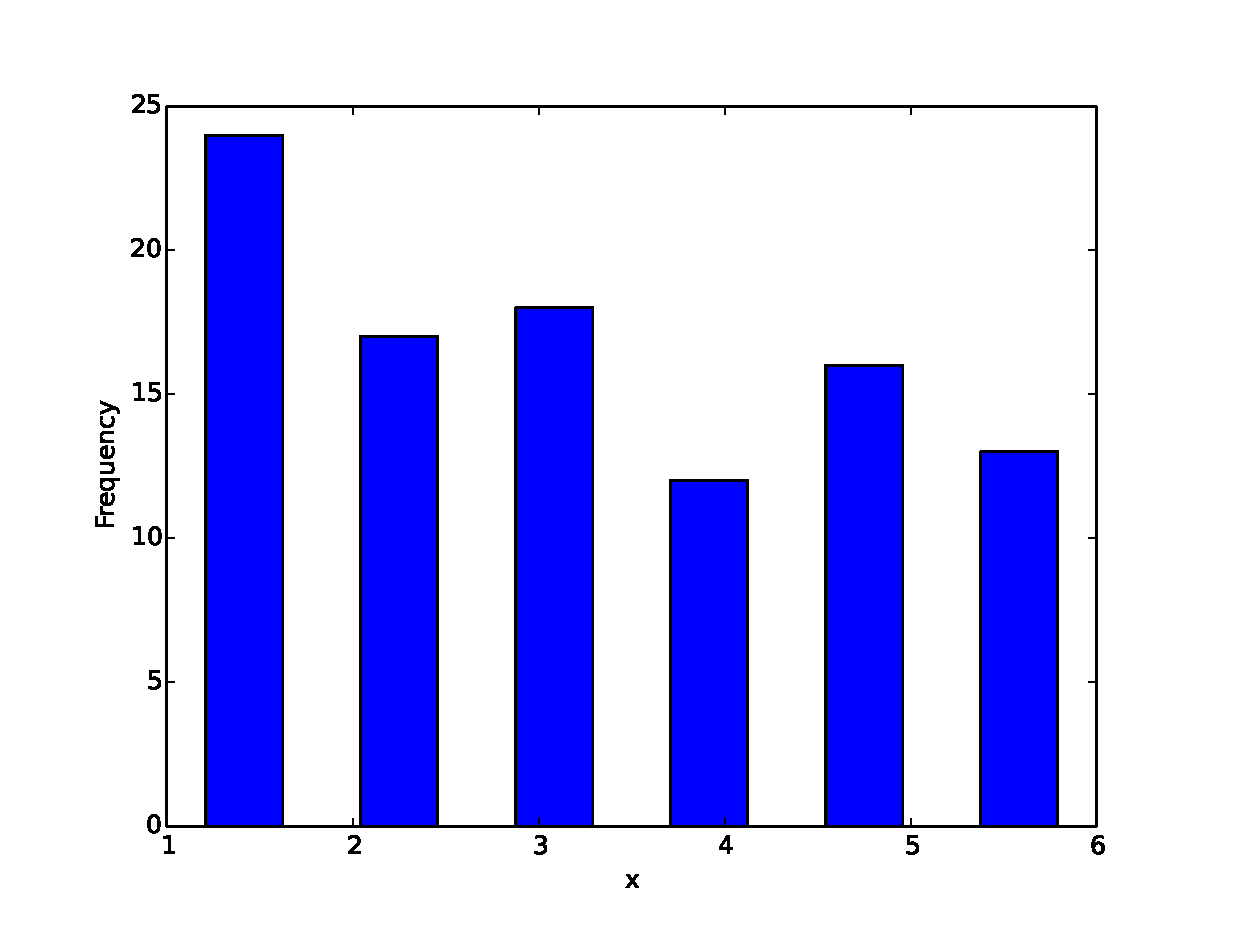
\includegraphics[width=0.5\linewidth]{DiscreteHist.eps}
}
\end{figure}
\end{frame}

\begin{frame}{Histograms of Continuous Variables I}  
 \begin{itemize} 
  \item First partition input space into a series of \emph{bins} $ I_1, \ldots, I_k$ 
  \begin{itemize} 
  \item Count the number of elements in each bin: $n_j = \sum_{x_i} \mathcal{I}\{x_i \in I_j\}$
  \item Plot in a bar graph $n_j$ for each $I_j$
  \end{itemize} 
  \item Alternatively, normalise to compute a density for each $I_j$: 
  \begin{displaymath} 
    h(y) = \frac{n_j}{n |I_j|} \quad \forall y \in I_j
  \end{displaymath}
 \end{itemize}
\end{frame}

\begin{frame}{Histograms of Continuous Variables II} 
\begin{itemize}
 \item E.g. the hypothetical distribution of heights in m of adult population  
\end{itemize}
\begin{figure}[htp]
\mbox{
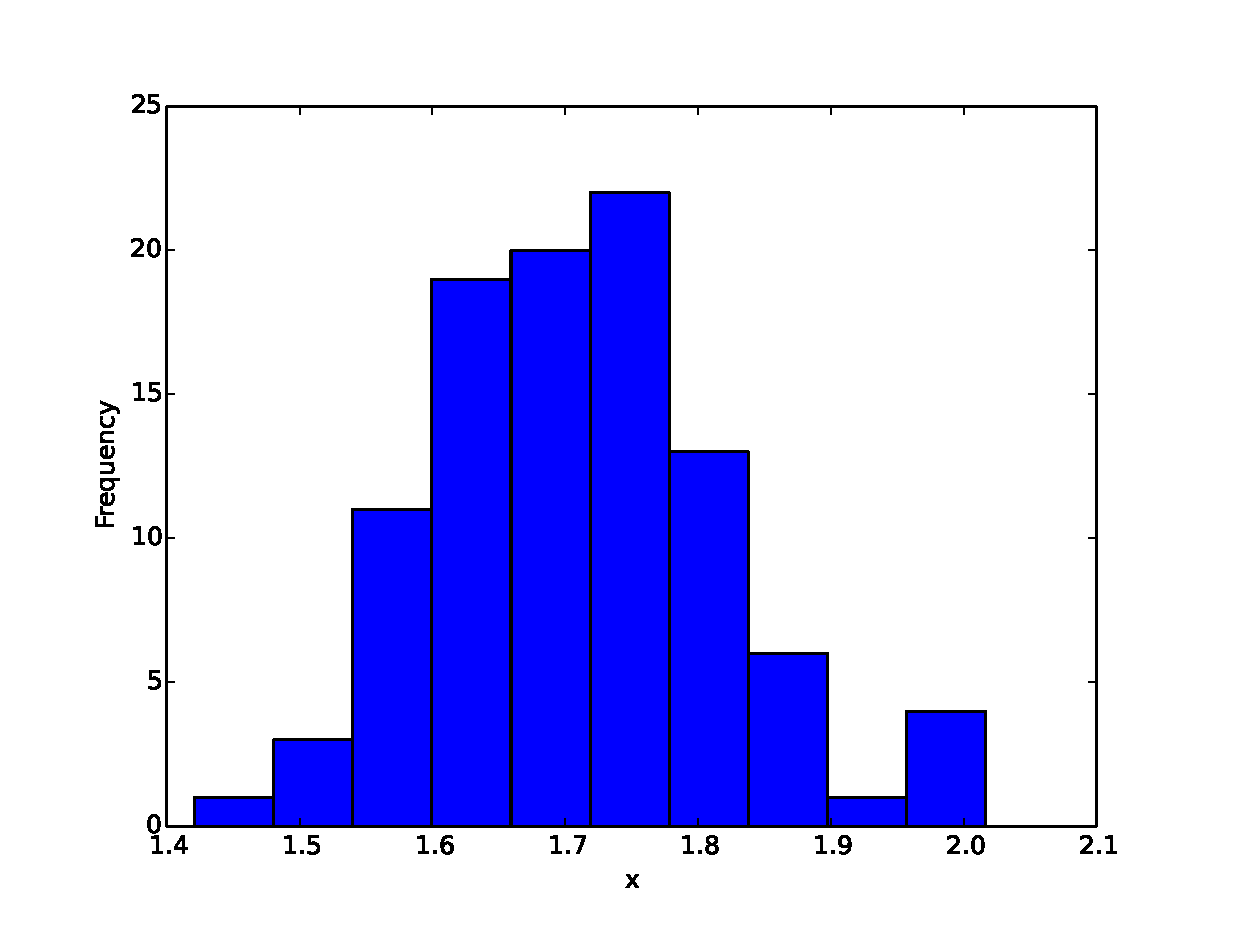
\includegraphics[width=0.5\linewidth]{ContinuousHist.eps}
}
\end{figure} 
\end{frame}

\begin{frame}{Cumulative Distribution Function}  
\begin{itemize} 
 \item Another representation of the distribution of values 
\item The cumulative distribution function is the proportion of values less than $x$
\begin{displaymath}
 F(x) = \frac{1}{n}\sum_{i=1}^n \mathcal{I}(x_i \leq x)
\end{displaymath}
\item The definition is the same for discrete and continuous variables 
\end{itemize}
 \begin{figure}[htp]
\mbox{
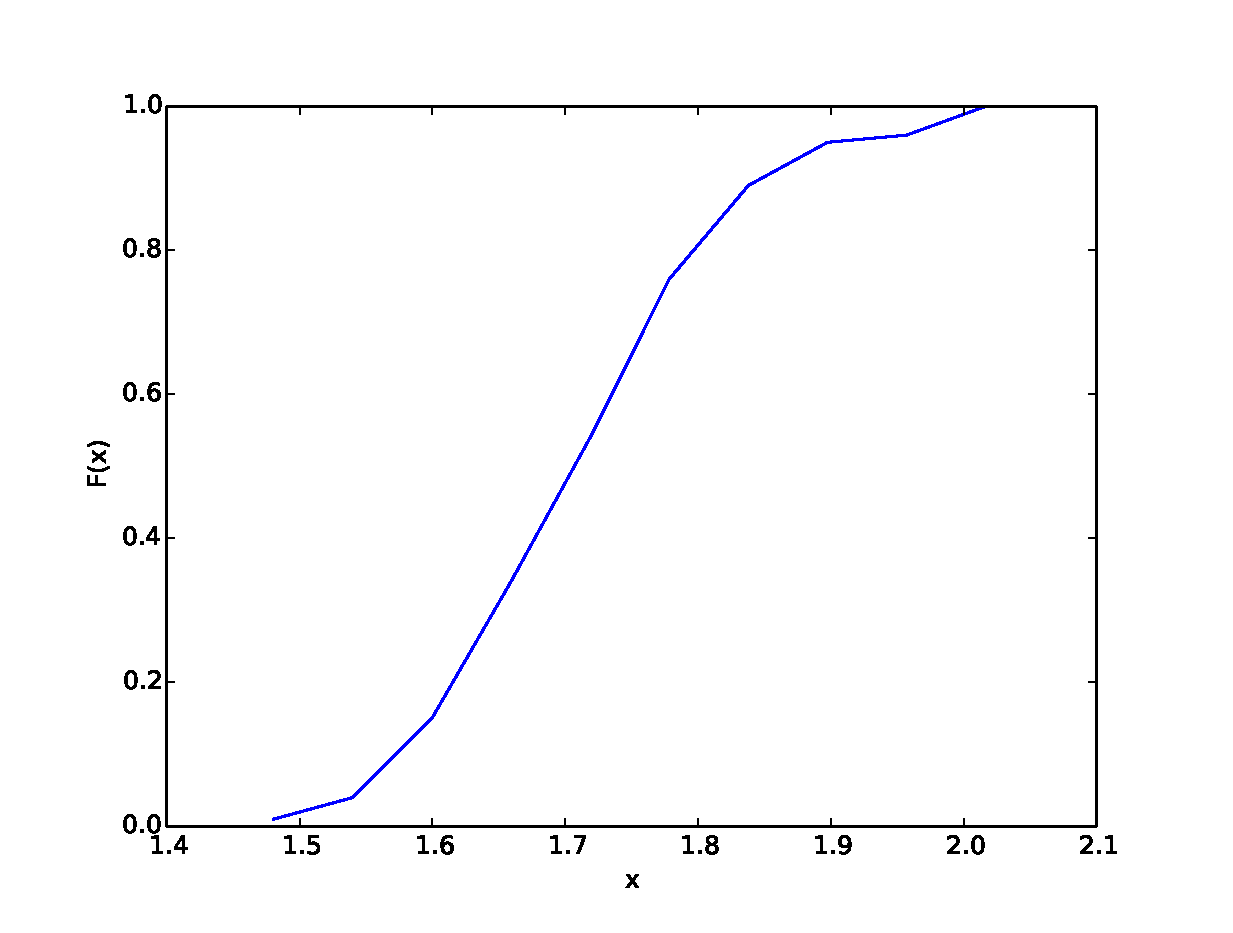
\includegraphics[width=0.5\linewidth]{ContinuousCDF.eps}
}
\end{figure} 
\end{frame}

\begin{frame}{Measures of Average}
\begin{itemize} 
 \item Look at statistics to summarise data $x_1, \ldots x_n$
  \item The \emph{mean} is defined as 
  \begin{displaymath}
   \bar{x} = \frac{1}{n}\sum_{i=1}^n x_i
  \end{displaymath}
\item The \emph{median} is the value such that $med(x)$ separates the higher half of the data from the lower half (if even number of samples take mean) 
\item The \emph{mode} $mod(x)$ is the most common value  
\end{itemize}
\end{frame}

\begin{frame}{Computing Averages} 
 \begin{itemize} 
  \item Example, tossing a die 20 times: 
\begin{table}
  \begin{tabular}{l | l l l l l l }
\hline 
  Outcome & 1 & 2 & 3 & 4 & 5 & 6 \\ 
  Frequency & 3 & 1 & 4 & 5 & 5 & 2 \\
\hline 
  \end{tabular} 
\end{table}
  \item Mean is 3.7 
  \item Median is 4 (mean of 10th and 11th value)
  \item Mode is 4 or 5 
 \end{itemize}
\end{frame}

\begin{frame}{Dispersion}  
\begin{itemize} 
 \item Gauge the variation in the values 
\begin{itemize} 
\item The \emph{variance} is the mean square difference with the mean 
\begin{displaymath} 
 var(x) = \frac{1}{n}\sum_{i=1}^n (x_i - \bar{x})^2
\end{displaymath}
 \item The \emph{standard deviation} is the root of the variance $std(x) = \sqrt{var(x)}$. 
\item Analogously the \emph{mean absolute deviation} is 
\begin{displaymath} 
  mad(x) = \frac{1}{n}\sum_{i=1}^n |x_i - med(x)|
\end{displaymath}
\end{itemize}
\end{itemize}
\end{frame}

\begin{frame}{Interquartile Range} 
 \begin{itemize} 
  \item Let $Q1$ be the median value less than $med(x)$ 
  \item Let $Q3$ be the median value greater than $med(x)$
  \item The \emph{interquartile range} is $Q3 - Q1$ 
  \begin{itemize}
  \item Represents 50\% of date in midrange  
  \end{itemize} 
 \end{itemize}
\end{frame}

\begin{frame}{Exercises}  
\begin{itemize} 
 \item Consider a set of numbers $x_1, \ldots x_n$. Show the following statements are true. 
\begin{itemize} 
\item The solution to minimising the objective for $a$ is the mean 
\begin{displaymath} 
 \mbox{min} \quad  \frac{1}{n}\sum_{i=1}^n (x_i - a)^2
\end{displaymath}
\item The solution to minimising the objective for $a$ is the median 
\begin{displaymath} 
 \mbox{min} \quad  \frac{1}{n}\sum_{i=1}^n |x_i - a|
\end{displaymath}
\end{itemize}
 \end{itemize}
\end{frame}

\begin{frame}{Order Statistics}  
\begin{itemize} 
 \item Often interesting in min/max values 
 \begin{displaymath} 
  x_{(1)} = \min_{1 \leq i \leq n} x_i, \quad x_{(n)} = \max_{1 \leq i \leq n} x_i
 \end{displaymath}
\item In general, the $k$th smallest value is $x_{(k)}$ 
\item In other words, let $(i_1, \ldots, i_n)$ be an ordering of indices from $\{1, \ldots, n\}$ 
\item The $k$th \emph{order statistic} is $x_{(k)} = x_{i_k}$
\end{itemize}
\end{frame}

\begin{frame}{Example}  
\begin{itemize} 
 \item Recap of tossing a die 
\end{itemize}

\begin{table}
  \begin{tabular}{l | l l l l l l }
\hline 
  Outcome & 1 & 2 & 3 & 4 & 5 & 6 \\ 
  Frequency & 3 & 1 & 4 & 5 & 5 & 2 \\
\hline 
  \end{tabular} 
\end{table}
\begin{itemize} 
 \item $x_{(6)} = 3$ and $x_{(1)} = 1$
\end{itemize}
\end{frame}

\begin{frame}{Quantiles} 
\begin{itemize} 
 \item For some value $\alpha \in (0, 1)$ we call the \emph{order quantile} $q_\alpha^x$ in which $x_{(m)}$ and $m = \lceil \alpha n \rceil$, where $\lceil \cdot \rceil$ means ceiling
 \item Follows that $Q_1 = q_{0.25}^x$, $med(x) = q_{0.5}^x$ and $Q_3 = q_{0.75}^x$
\end{itemize}
\end{frame}

\begin{frame}{Boxplots I} 
\begin{itemize} 
 \item A visual representation of key measures in a set of numbers $(A, Q1, med(x), Q3, B)$ 
 \item Items outside $A, B$ are considered outliers 
 \item $Q1, med(x), Q3$ are the first quartile, median and third quartile 
\end{itemize}
  \begin{figure}[htp]
\mbox{
\includegraphics[width=0.5\linewidth]{BoxPlot.eps}
}
\end{figure} 
\end{frame}

\begin{frame}{Boxplots II} 
\begin{itemize} 
 \item $A = \min \{x_i : x_i \geq Q1 - 1.5\Delta \}$ and $B = \max\{x_i : x_i \leq Q3 + 1.5\Delta \}$ with $\Delta = Q3 - Q1$
 \item For the normal distribution, the probability of a value outside of $[A, B]$ is $0.7\%$
 \item Half the values are found in the box (between $Q1$ and $Q3$) 
 \item Half the values are to the left of median (same for right)
 \item If no outliers, all values are in $[A, B]$
 \item A symmetric distribution has a symmetric box
 \item Boxplots are useful for comparing two distributions 
\end{itemize}
\end{frame}

\begin{frame}{Skewness}  
\begin{itemize} 
 \item The extent a distribution leans to one side of mean is \emph{skewness} 
\begin{displaymath} 
 \alpha_x = \frac{1}{ns^3_x} \sum_{i=1}^n (x_i - \bar{x})^3
\end{displaymath}
Positive skew if right tail is longer, negative if left tail is longer 
\item Shape of peaks and tails is called \emph{kurtosis} (excess kurtosis):
\begin{displaymath} 
 \beta_x = \frac{1}{ns^4_x} \sum_{i=1}^n (x_i - \bar{x})^4 - 3
\end{displaymath}
High kurtosis distribution has sharper peak and fatter tails. Low kurtosis distribution ha more rounded peak with wider tails. 
\end{itemize}
 
\end{frame}


\begin{frame}{Exercise}  
\begin{itemize} 
 \item Polychlorinated biphenyls (PCBs) are toxic organic compounds used in electronics and cooling systems. 
 \item Two samples representing contamination in soil ($10^{-4}$g/kg)
 \begin{itemize}
 \item Rural: 3.5 1 1.6 12 8.1 5.3 23 8.2 1.8 9.8 1.5 9.7 9 15
 \item Urban: 24 11 107 18 29 49 94 12 16 22 
 \end{itemize}
 \item Draw the boxplots for these two samples and comment on the results
\end{itemize}
\end{frame}

\begin{frame}{Covariance and Correlation}
\begin{itemize} 
 \item Consider two samples $x_1, \ldots, x_n$ and $y_1, \ldots, y_n$. 
  \item The \emph{covariance}
 \begin{displaymath} 
  s_{xy} = \frac{1}{n} \sum_{i=1}^n (x_i - \bar{x})(y_i - \bar{y}) 
 \end{displaymath}
  where $\bar{x}$ and $\bar{y}$ are means 
 \item The \emph{correlation coefficient} $\in [-1, +1]$ is 
 \begin{displaymath}
  \rho_{xy} = \frac{s_{xy}}{\sqrt{s_{xx}s_{yy}}}
 \end{displaymath}
  where $\sqrt{s_{xx}}$ is the standard deviation. 
 \item We say correlation is zero if either sample has s.d. 0 
 \item If $|\rho_{xy}| = 1$ then $x, y$ have an affine relationship $x_i = a y_i + b$ 
\end{itemize}
\end{frame}

\begin{frame}{Scatter Plots} 
\begin{itemize}
 \item A \emph{scatter plot} represents the locations of two samples $x_1, \ldots, x_n$ and $y_1, \ldots, y_n$ in space as the coordinates $(x_1, y_1), \ldots, (x_n, y_n)$ 
 \item Example: 
\end{itemize}
  \begin{figure}[htp]
\mbox{
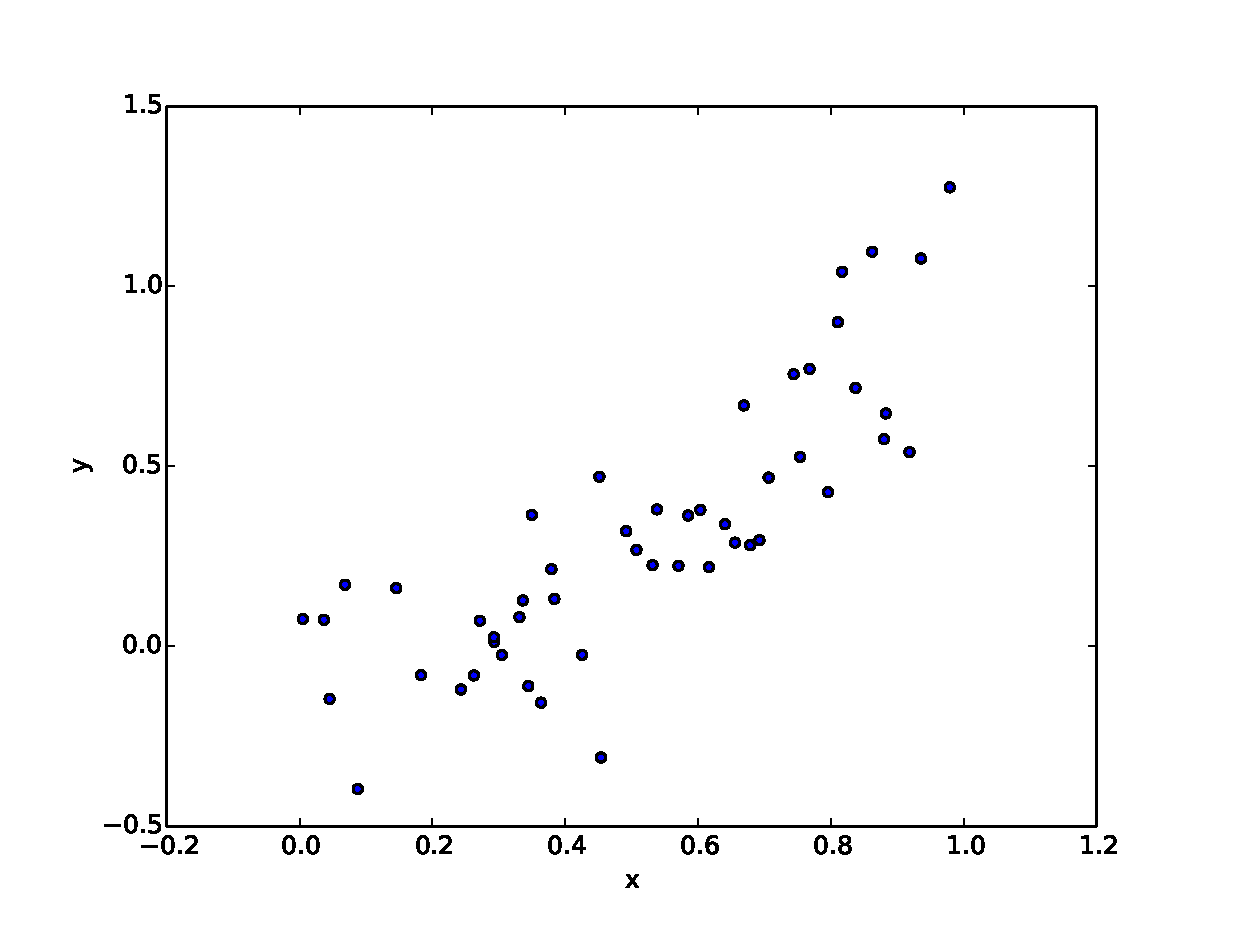
\includegraphics[width=0.5\linewidth]{ScatterPlot.eps}
}
\end{figure} 
\end{frame}

\begin{frame}{Linear Regression} 
\begin{itemize} 
 \item Linear regression models a linear relationship between $x_1, \ldots, x_n$ and $y_1, \ldots, y_n$ using $y = ax + b$ 
 \begin{displaymath} 
  \min_{a, b} \sum_{i=1}^n (y_i  - a x_i - b)^2 
 \end{displaymath}
 is solved using $a = \frac{s_{xy}}{s_{xx}} \quad b = \bar{y} - a\bar{x}$
 \item This is known as \emph{least squares regression}
\item Linear regression of $X$ onto $Y$ does not in general coincide with $Y$ onto $X$ 
 \end{itemize}
\end{frame}

\begin{frame}{QQ Plots} 
\begin{itemize}
 \item A Q–Q plot (Q stands for quantile) is a plot of two distributions according to the order quantiles $q_\alpha^x$ and $q_\alpha^y$
 \item Two applications 
 \begin{itemize}
 \item Compare data within quantiles for a distribution to a theoretical one 
 \item Compare two data samples 
 \end{itemize}
 \item If the gradient of the plot is approximately 1 and points align, the distribution are equal 
 \item If points align, but the gradient is not 1, one distribution is a transformation of the other 
\end{itemize}
\end{frame}

\begin{frame}{QQ Plots Example}  
\begin{itemize}
 \item Draw 1000 points from $\mathcal{N}(0, 1)$ and $\mathcal{N}(0, 0.2)$ 
\item Order points and plot $q_\alpha^x$ with $q_\alpha^y$
\end{itemize}

   \begin{figure}[htp]
\mbox{
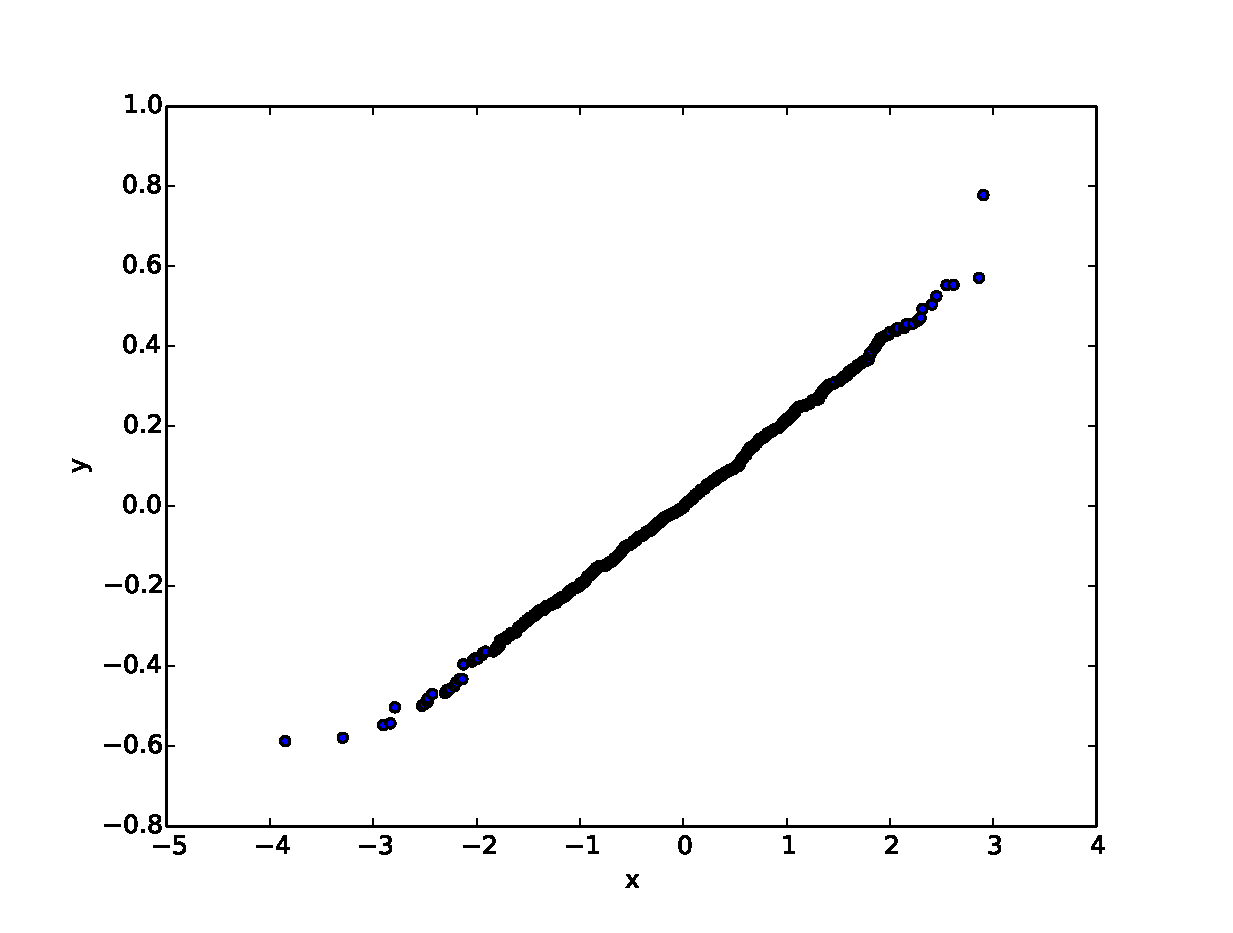
\includegraphics[width=0.5\linewidth]{QQPlot.eps}
}
\end{figure} 
\end{frame}

\begin{frame}{Summary} 
\begin{itemize} 
 \item Discrete and continuous variables, histograms  
 \item Cumulative distribution function 
\item Averages - means, modes, medians 
\item Divergence properties - variance, quartiles, box plots  
\item Covariance, correlation of two variables
\item Linear regression 
\item Scatter, QQ plots to visualise paired observations 
\end{itemize}
\end{frame}


\begin{frame}{The End} 
Thanks for listening!  
\end{frame}


\end{document}
